\begin{frame}
\frametitle{Das Mock-System}


\onslide<2->{
\begin{itemize}
	\onslide<1->{\item Wird genutzt, wenn mit Geräten kommuniziert wird:	
	\begin{itemize}
		\item \texttt{mock\_system.write\_to\_AWG}
		\item \texttt{mock\_system.read\_from\_DSO}
	\end{itemize}		
 	}
	\onslide<3->{\item Simuliert das Verhalten des Messaufbaus nach dem Hammerstein Model}
\end{itemize}
}

\only<4-6>{
		\begin{textblock}{20}(13,37)
    		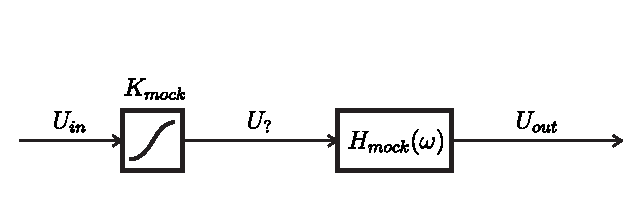
\includegraphics[]{slides/ResultCode/Slide_mock.eps} 
		\end{textblock}		
}
\only<5-6>{
		\begin{textblock}{20}(21,64)
    		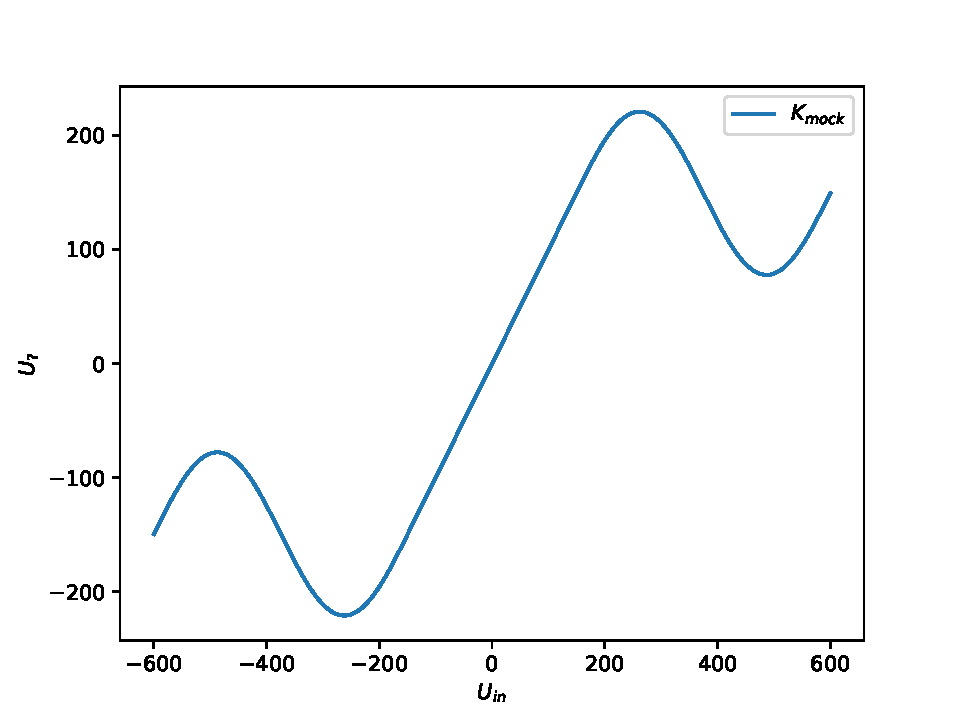
\includegraphics[ width=2.9cm, height=2.4cm ]{slides/ResultCode/plots/K_mock.pdf} 
		\end{textblock}			
}
\only<6>{	
		\begin{textblock}{20}(62,64)
    		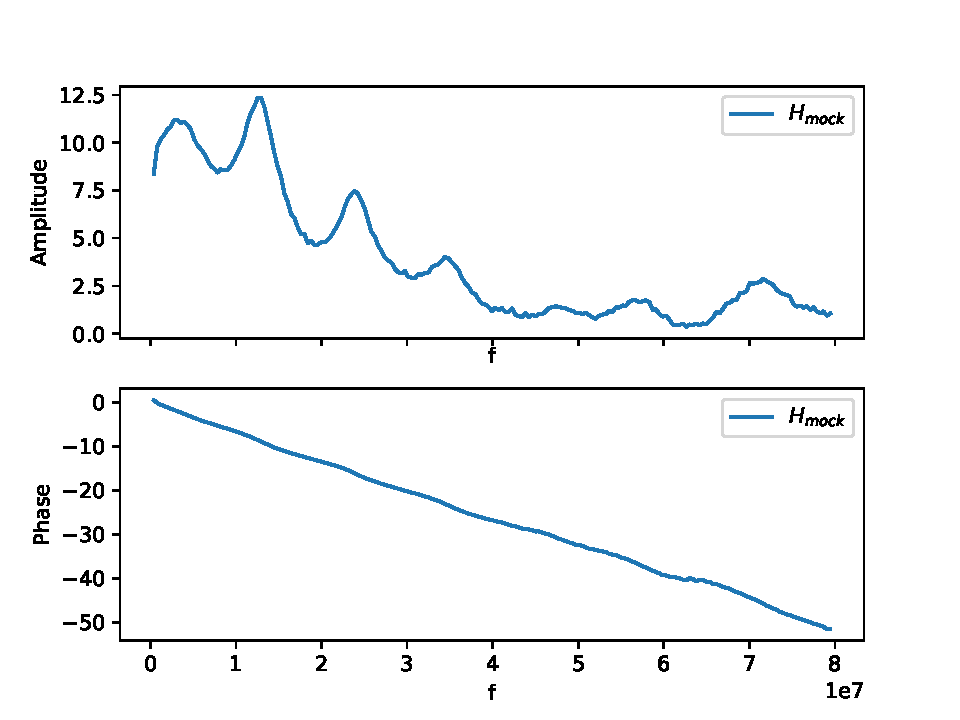
\includegraphics[ width=2.9cm, height=2.4cm]{slides/ResultCode/plots/H_mock.pdf} 
		\end{textblock}	
}



\onslide<7->{Vorteile:
\onslide<8->{
\begin{itemize}
	\onslide<8->{\item Ermöglicht:	
	\begin{itemize}
			\onslide<8->{\item Unit Tests von Bausteinen, in den Gerätekommunikation stattfindet }
			\onslide<9->{\item System Tests }	
			\onslide<10->{\item Testen von Randfällen}
	\end{itemize}		
 	}
	\onslide<11->{\item Hilft das System besser zu verstehen }
\end{itemize}
}
} 

\onslide<12->{Nachteile:
\onslide<12->{
\begin{itemize}
	\onslide<12->{\item Extra Aufwand: mehr Code zu debuggen}
\end{itemize}
}
}
 
 

\end{frame}
